\documentclass[landscape]{article}
\usepackage[pdftex]{graphicx,color}
\pagestyle{empty}
\oddsidemargin  -0.5 in
\evensidemargin -0.5 in
\headheight     0 in
\topmargin      -1 in
\textheight     7.7 in
\textwidth      10 in
\begin{document}
\huge
\renewcommand{\labelitemi}{-}
\setlength{\parindent}{0 cm}

\mbox{ }

\vfill
\begin{minipage}{\linewidth}
\begin{center}
{\Huge Progress on the $\Gamma_{ee}$ Efficiency Measurement}

\vspace{1.5 cm}
Jim Pivarski

\vspace{1.5 cm}
\today
\end{center}
\end{minipage}
\vfill
\pagebreak

\begin{center}
  \includegraphics[width=\linewidth]{/cdat/daf9/mccann/neweff/gaudy_slide.pdf}
\end{center}

{\Huge Remember $\Gamma_{ee}$?}

\begin{itemize}

  \item data16--27 included 21 lineshape scans of $\Upsilon(1S)$, $\Upsilon(2S)$, $\Upsilon(3S)$

  \item Statistical uncertainties are negligible $\sim$0.4\%

  \item Background systematics reduced to $\sim$0.2\%

  \item Efficiency measurement currently limited by a data/MC disagreement ($\sim$1.7\%)

  \item Luminosity and energy-wiggle studies to follow.

\end{itemize}
\vfill
\begin{center}
  \includegraphics[width=0.9\linewidth]{p2gg_three_peaks.pdf}
\end{center}

\pagebreak

{\Huge Analysis cuts}

\begin{center}
\includegraphics[width=\linewidth]{cuts0.pdf}
\end{center}
\vfill

To loosen these cuts, I will need to get raw data
\vfill
\pagebreak

{\Huge Analysis cuts}

\begin{center}
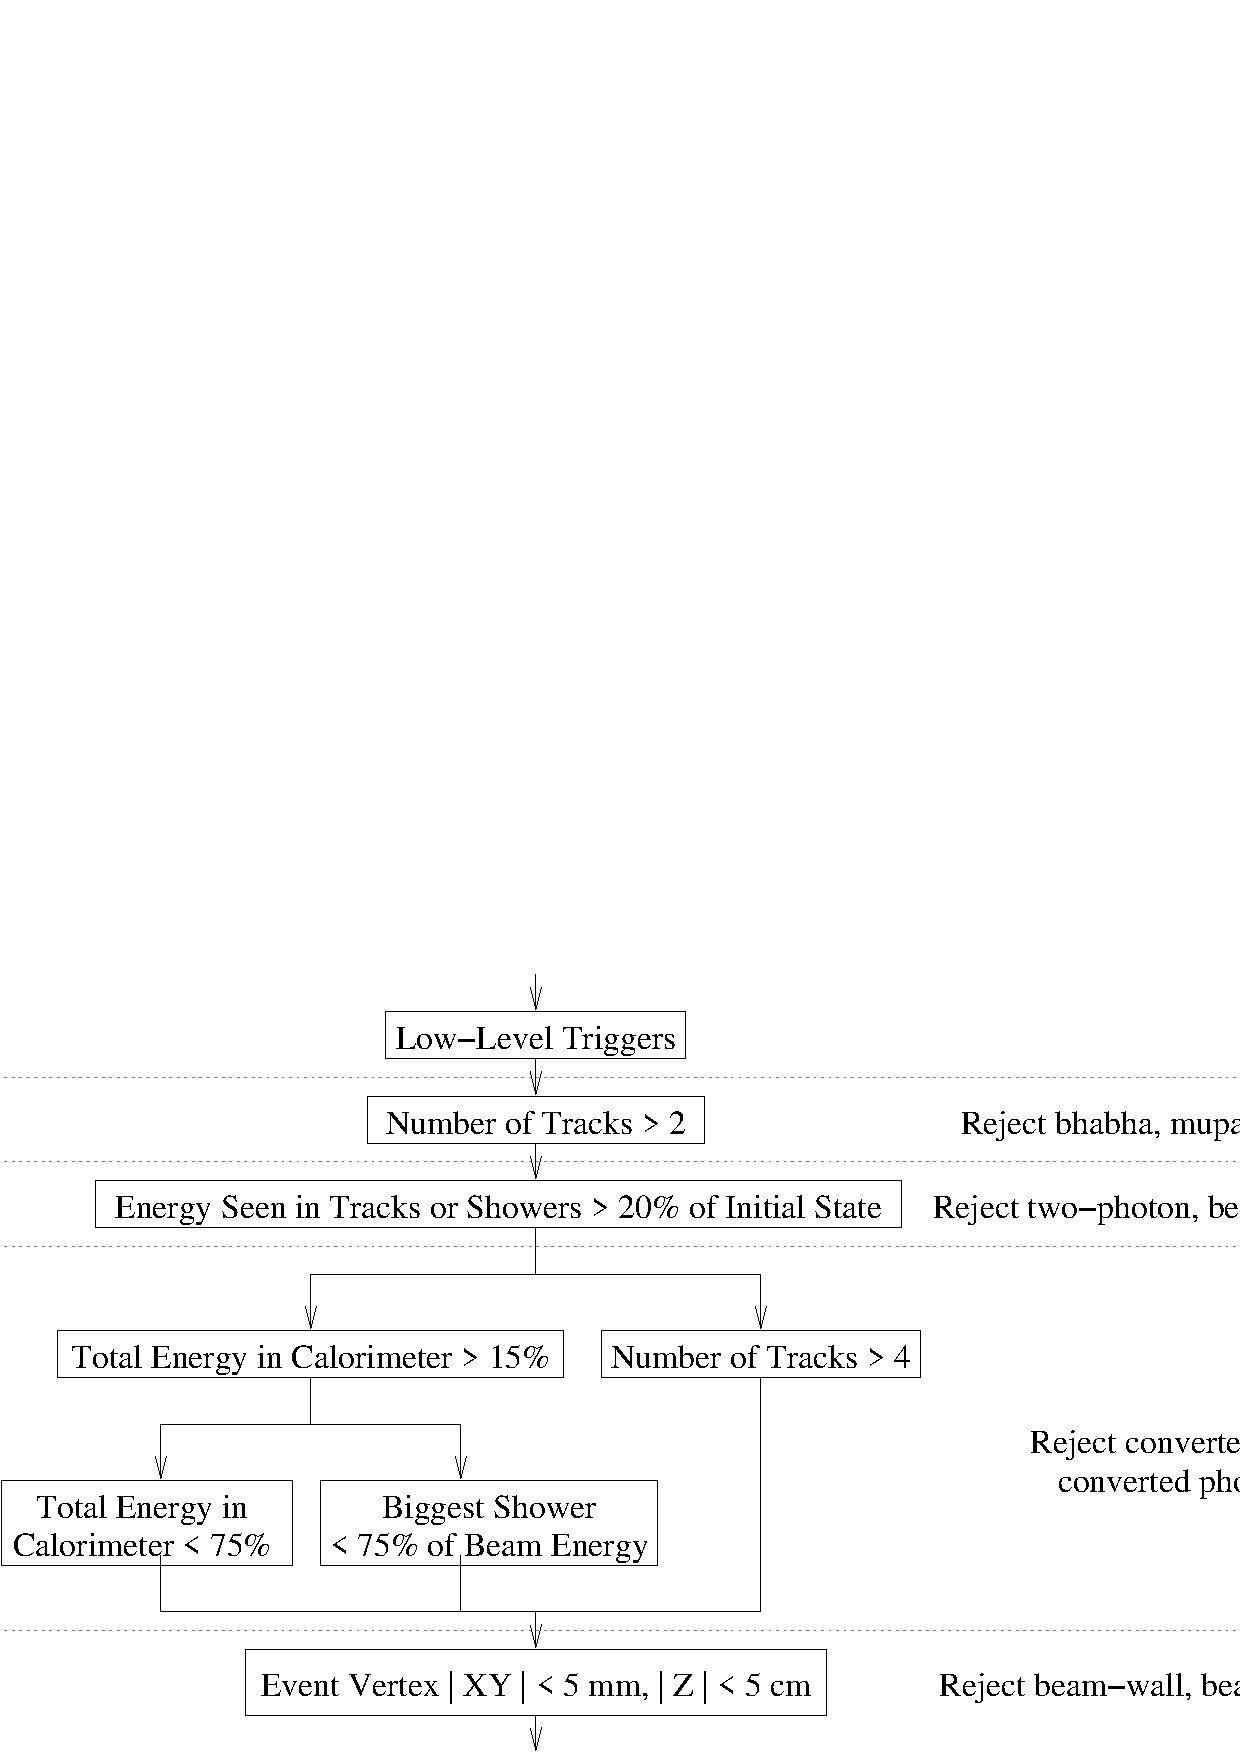
\includegraphics[width=\linewidth]{cuts.pdf}
\end{center}
\vfill

To loosen these cuts, I will need to get raw data
\vfill
\pagebreak

{\Huge Comparing raw data with resonance Monte Carlo}

\vfill
\begin{center}\begin{minipage}{0.85\linewidth}
Raw data contains continuum processes (bhabhas, two-photon, continuum
hadrons) which will need to be removed by a continuum subtraction.

\vspace{1 cm}
That subtraction will have more statistical power if some large
continuum processes are first cut.

\vspace{1 cm}
The three remaining backgrounds--- beamgas, beamwall, and cosmic
rays--- will need to be cut out in any case.
\end{minipage}\end{center}

\vfill
{\Huge Efficiency cuts}

\begin{center}
\includegraphics[width=\linewidth]{reffcuts0.pdf}
\end{center}
\vfill
\pagebreak

{\Huge Analysis cuts}

\begin{center}
\includegraphics[width=\linewidth]{cuts2.pdf}
\end{center}
\vfill

{\Huge Efficiency cuts}

\begin{center}
\includegraphics[width=\linewidth]{reffcuts2.pdf}
\end{center}
\vfill
\pagebreak

{\Huge Now I can finally show you the data/MC disagreement}

\vspace{1 cm}
Continuum-subtracted $\Upsilon(2S)$ with efficiency cuts
\vspace{-1 cm}

\begin{center}
\includegraphics[height=0.9\textheight]{comp_tracks1.pdf}
\end{center}
\pagebreak

{\Huge Now I can finally show you the data/MC disagreement}

\vspace{1 cm}
EvtGen improves low multiplicity agreement
\vspace{-1 cm}

\begin{center}
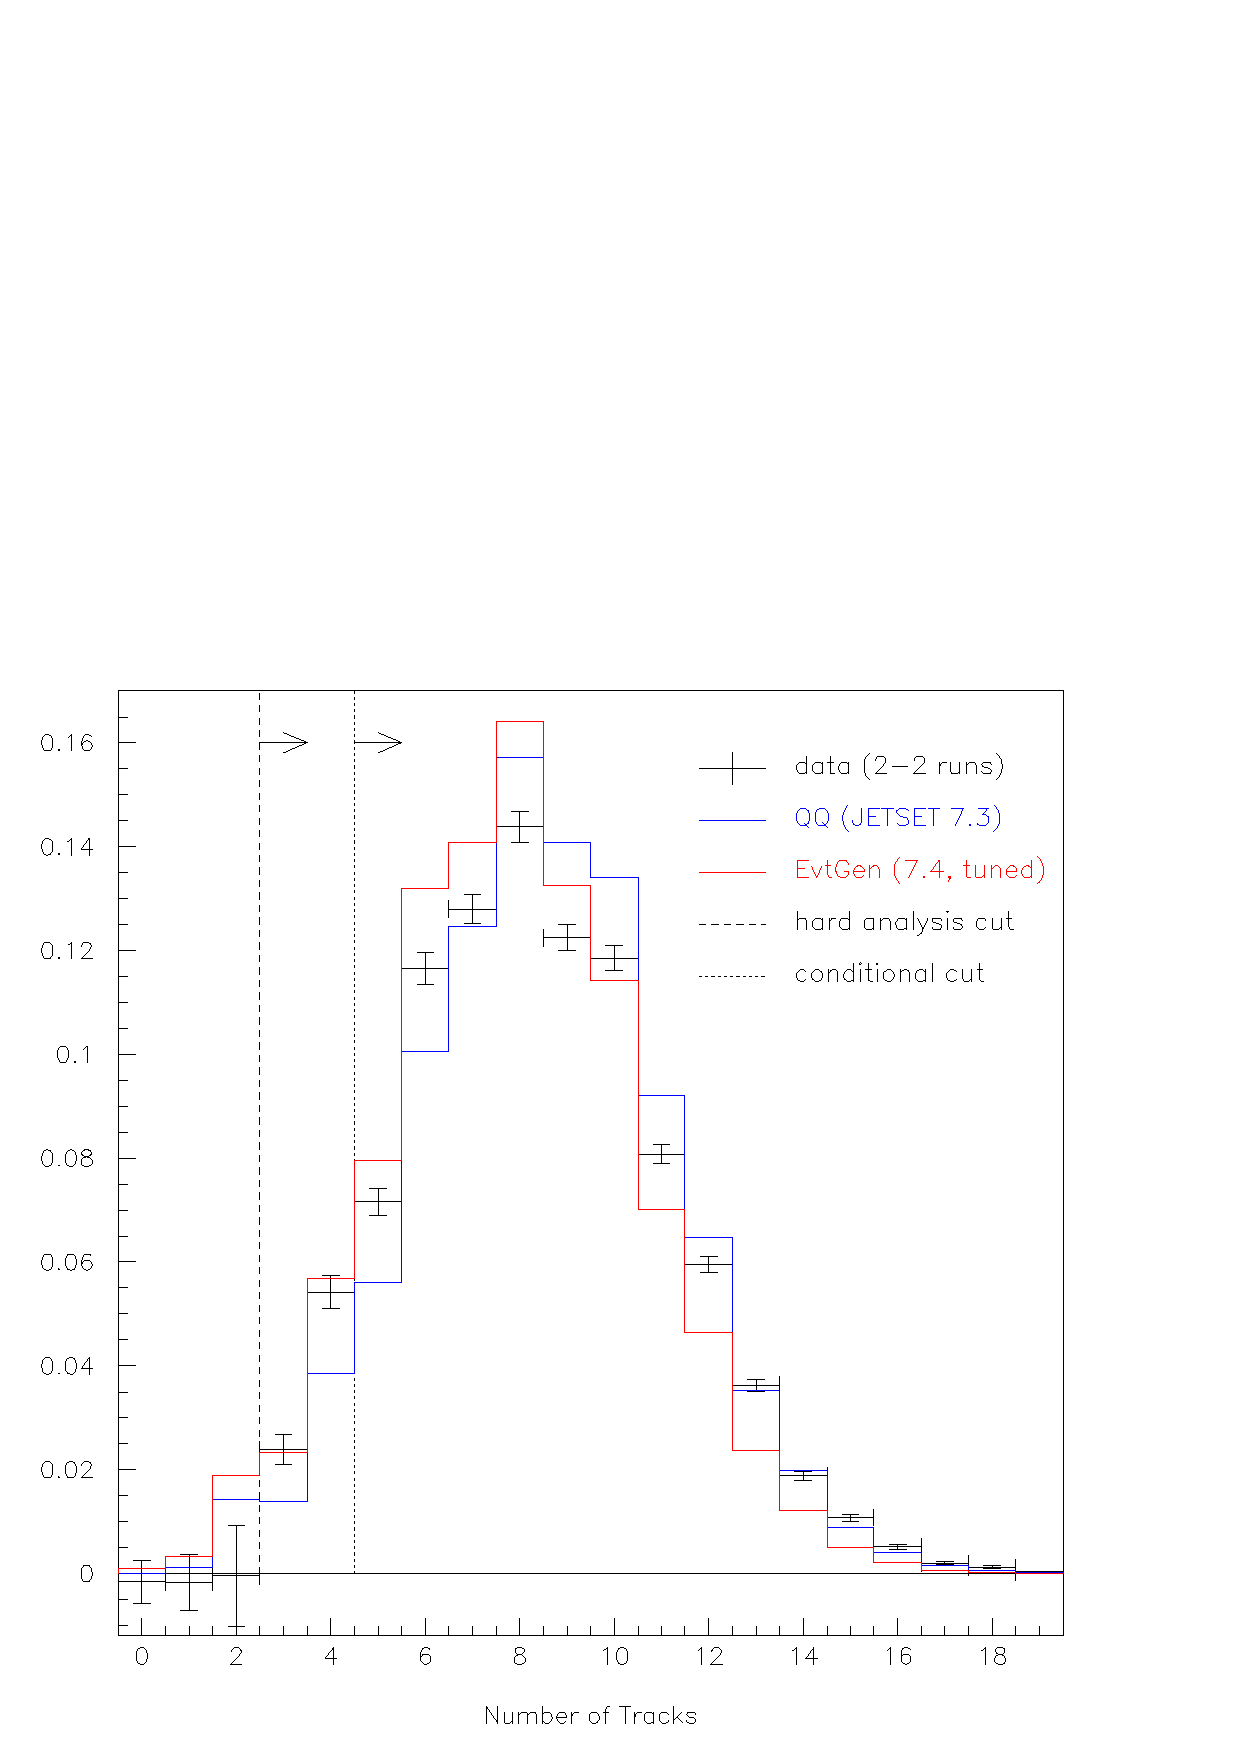
\includegraphics[height=0.9\textheight]{comp_tracks2.pdf}
\end{center}
\pagebreak

{\Huge Maybe I can use the raw data to measure efficiency}

\vfill
Events that pass the efficiency cut and continuum subtraction are
almost all $\Upsilon$ events.  (Beamgas/wall/cosmic are controlled
just as they were for the background study).

\vfill
In fact, they are almost all one kind of $\Upsilon$ decay:
\vspace{0.25 cm}
\begin{center}
  \begin{tabular}{c c}
    \vspace{0.25 cm}
    \hspace{0.25 cm} Class of decays \hspace{0.25 cm} & \hspace{0.25 cm} Fraction that pass efficiency cut \hspace{0.25 cm} \\\hline
    \vspace{-0.5 cm}
    & \\
    \vspace{0.25 cm}
    \hspace{0.25 cm} $\Upsilon \to$ all hadrons or $\tau^+ \tau^-$ \hspace{0.25 cm} & \hspace{0.25 cm} 99\% \hspace{0.25 cm} \\
    \vspace{0.25 cm}
    \hspace{0.25 cm} $\Upsilon \to \ldots \to X \ell^+ \ell^-$ \hspace{0.25 cm} & \hspace{0.25 cm} 5\% \hspace{0.25 cm}
  \end{tabular}
\end{center}

\vfill
\begin{center}
\includegraphics[width=\linewidth]{reffcuts0.pdf}
\end{center}
\vfill
\pagebreak

\hspace{1.5 cm}
\begin{minipage}{8 in}
\Large

\vspace{0.7 cm}
\begin{tabular}{p{4.6 in} p{2 in} p{1.3 in}}
Decay Mode & Branching Ratio & Uncertainty \\ \hline
$   \Upsilon(1S) \to e^+ e^-                      $ & $   0.0251   $ & $   0.00050   $ \\ 
$   \Upsilon(1S) \to \mu^+ \mu^-                  $ & $   0.0251   $ & $   0.00050   $ \\\hline\hline
$   \Upsilon(1S) \to \ldots \to X \ell^+ \ell^-   $ & $   0.0502   $ & $   0.0010    $ \\\hline
\end{tabular}

\vspace{1 cm}
\begin{tabular}{p{4.6 in} p{2 in} p{1.3 in}}
Decay Mode & Branching Ratio & Uncertainty \\ \hline
$   \Upsilon(2S) \to e^+ e^-                                                        $ & $   0.0125      $ & $   0.0014     $ \\ 
$   \Upsilon(2S) \to \mu^+ \mu^-                                                    $ & $   0.0125      $ & $   0.0014     $ \\ 
$   \Upsilon(2S) \to \pi^+ \pi^- \Upsilon(1S) \to e^+ e^-                           $ & $   0.00472     $ & $   0.00018    $ \\ 
$   \Upsilon(2S) \to \pi^+ \pi^- \Upsilon(1S) \to \mu^+ \mu^-                       $ & $   0.00472     $ & $   0.00018    $ \\ 
$   \Upsilon(2S) \to \pi^0 \pi^0 \Upsilon(1S) \to e^+ e^-                           $ & $   0.00226     $ & $   0.00020    $ \\ 
$   \Upsilon(2S) \to \pi^0 \pi^0 \Upsilon(1S) \to \mu^+ \mu^-                       $ & $   0.00226     $ & $   0.00020    $ \\ 
$   \Upsilon(2S) \to \gamma \chi_{b0}(1P) \to \gamma \Upsilon(1S) \to e^+ e^-       $ & $   0.0000573   $ & $   8.6 \times 10^{-6}  $ \\ 
$   \Upsilon(2S) \to \gamma \chi_{b0}(1P) \to \gamma \Upsilon(1S) \to \mu^+ \mu^-   $ & $   0.0000573   $ & $   8.6 \times 10^{-6}  $ \\ 
$   \Upsilon(2S) \to \gamma \chi_{b1}(1P) \to \gamma \Upsilon(1S) \to e^+ e^-       $ & $   0.000598    $ & $   0.00015    $ \\ 
$   \Upsilon(2S) \to \gamma \chi_{b1}(1P) \to \gamma \Upsilon(1S) \to \mu^+ \mu^-   $ & $   0.000598    $ & $   0.00015    $ \\ 
$   \Upsilon(2S) \to \gamma \chi_{b2}(1P) \to \gamma \Upsilon(1S) \to e^+ e^-       $ & $   0.000387    $ & $   0.000078   $ \\ 
$   \Upsilon(2S) \to \gamma \chi_{b2}(1P) \to \gamma \Upsilon(1S) \to \mu^+ \mu^-   $ & $   0.000387    $ & $   0.000078   $ \\\hline\hline
$   \Upsilon(2S) \to \ldots \to X \ell^+ \ell^-                                     $ & $   0.0410      $ & $   0.0030     $ \\\hline
\end{tabular}

\vspace{1 cm}
\begin{tabular}{p{4.6 in} p{2 in} p{1.3 in}}
Decay Mode & Branching Ratio & Uncertainty \\\hline
$   \Upsilon(3S) \to e^+ e^-                                                                                           $ & $   0.0181      $ & $   0.0017     $ \\ 
$   \Upsilon(3S) \to \mu^+ \mu^-                                                                                       $ & $   0.0181      $ & $   0.0017     $ \\ 
$   \Upsilon(3S) \to \pi^+ \pi^- \Upsilon(1S) \to e^+ e^-                                                              $ & $   0.00113     $ & $   0.000058   $ \\ 
$   \Upsilon(3S) \to \pi^+ \pi^- \Upsilon(1S) \to \mu^+ \mu^-                                                          $ & $   0.00113     $ & $   0.000058   $ \\
\hspace{2 cm} (68 more\ldots) & \hspace{0.25 cm} $\ddots$ & \hspace{0.25 cm} $\ddots$ \\\hline\hline
$   \Upsilon(3S) \to \ldots \to X \ell^+ \ell^-                                                    $ & $   0.0444      $ & $   0.0034     $ \\\hline
\end{tabular} \\
\end{minipage}

% intentionally left un \pagebreak ed

\begin{center}
  \begin{tabular}{p{0.5\linewidth} p{0.48\linewidth}}
    \begin{minipage}{\linewidth}
      \vspace{-0.4 cm}
      \includegraphics[width=\linewidth]{breakdown.pdf}
    \end{minipage} &
    \begin{minipage}{\linewidth}
      \LARGE

\vspace{-2.5 cm}
\[ \mbox{uncorrected efficiency} = \frac{\mbox{data ``Pass Analysis''}}{\mbox{data ``Pass Efficiency''}} \]
Uncertainties: 
\begin{itemize}
  \item 0.66\% counting statistics
  \item 5.0\% from int.\ luminosity {\it statistical error}
\end{itemize}

Numerator (multiplicative) corrections:
\[ (1 - \mbox{PDG})\, \mbox{\color{blue} 0.18\%} + (\mbox{PDG})\, \mbox{1.10\%}\mbox{, or} \]
\[ (1 - \mbox{PDG})\, \mbox{\color{red} 0.30\%} + (\mbox{PDG})\, \mbox{1.10\%} \]

Denominator (multiplicative) corrections:
\[ (1 - \mbox{PDG})\, \mbox{\color{blue} 99.60\%} + (\mbox{PDG})\, \mbox{4.97\%}\mbox{, or} \]
\[ (1 - \mbox{PDG})\, \mbox{\color{red} 99.48\%} + (\mbox{PDG})\, \mbox{4.97\%} \]

Uncertainties:
\begin{itemize}
  \item Numerator uncertainties are negligible
  \item 0.28\% from PDG branching fraction
  \item 0.34\% from choice of MC generator
\end{itemize}

\vspace{0.3 cm}
\begin{center}\fbox{\begin{minipage}{0.75\linewidth}
\begin{center}
$\pm$5.0\% statistical $\pm$0.44\% systematic \\
$\pm$ small background contribution
\end{center}
\end{minipage}}\end{center}

    \end{minipage}
  \end{tabular}
\end{center}

\pagebreak

{\Huge Why am I not giving you a number? (Conclusions Slide)}

\begin{enumerate}
  \vfill
  \item The 5\% uncertainty contribution from int.\ luminosity statistics

  \vfill
  The int.\ luminosity fraction between peak and continuum is known to
  $\pm$1.6\% (in this sample), but appears between large numbers:

\[ \frac{\mbox{``Pass Analysis''}_{\mbox{\large peak}} - \mbox{``Pass Analysis''}_{\mbox{\large continuum}}
   \times (\mbox{int.\ luminosity fraction})}
   {\mbox{``Pass Efficiency''}_{\mbox{\large peak}} - \mbox{``Pass Efficiency''}_{\mbox{\large continuum}}
   \times (\mbox{int.\ luminosity fraction})} \]

  \vfill
  If int.\ luminosity fraction is known to $\pm$0.16\%, it would
  have a 0.5\% impact on the final result.

  \vfill
  This uncertainty can be minimized by adding more data {\it and} by
  optimizing the $e^+e^- \to \gamma \gamma$ cuts.  For this
  sub-analysis, an energy-indepdendent systematic error in the int.\
  luminosity measurement doesn't matter.

  \vfill
  \item I need to look at single-beam runs again to quantify the
  impact of beamgas, beamwall, and cosmic rays.

  \vfill
  \item I'm not certain I understand what defines a failed trigger.

  \vfill
\end{enumerate}

\end{document}







%% {\Huge Area of each peak is related to $\Gamma_{ee}$}

%% \[
%% \begin{array}{r c l}
%% \Gamma(\Upsilon \to e^+ e^-) &=& \displaystyle \frac{\mbox{$M_\Upsilon$}^2}{6 \pi^2} \mbox{ }
%% \int dE\, \sigma(e^+ e^- \to \Upsilon) \\
%% \Gamma(\Upsilon \to e^+ e^-) &=& \displaystyle \frac{\mbox{$M_\Upsilon$}^2}{6 \pi^2} \mbox{ }
%% \frac{\Gamma_{\mbox{\normalsize tot}}}{\Gamma_{\mbox{\normalsize had}}} \mbox{ }
%% \int dE\, \sigma(e^+ e^- \to \Upsilon \to \mbox{hadrons}) \\
%% \Gamma(\Upsilon \to e^+ e^-) &=& \displaystyle \frac{\mbox{$M_\Upsilon$}^2}{6 \pi^2} \mbox{ }
%% \frac{\Gamma_{\mbox{\normalsize tot}}}{\Gamma_{\mbox{\normalsize whatever}}} \mbox{ }
%% \int dE\, \sigma(e^+ e^- \to \Upsilon \to \mbox{whatever})
%% \end{array}
%% \]

%% \vfill
%% \begin{center}
%% \begin{tabular}{p{0.02\linewidth} p{0.50\linewidth}}
%%   \begin{minipage}{\linewidth}
%%     \rotatebox{90}{$\sigma(e^+e^- \to \mbox{hadrons})$ (nb)}
%%   \end{minipage} &
%%   \begin{minipage}{\linewidth}
%%     \includegraphics[width=\linewidth]{plot_em_all2_revision_wide2.pdf}
%%   \end{minipage} \\
%%   & \centering Energy (MeV)
%% \end{tabular}
%% \end{center}
